\markboth{}{}
%insertion de l'image de fond du dos (resume)
%background image for resume (back)
 \AddToShipoutPicture*{\put(0,0){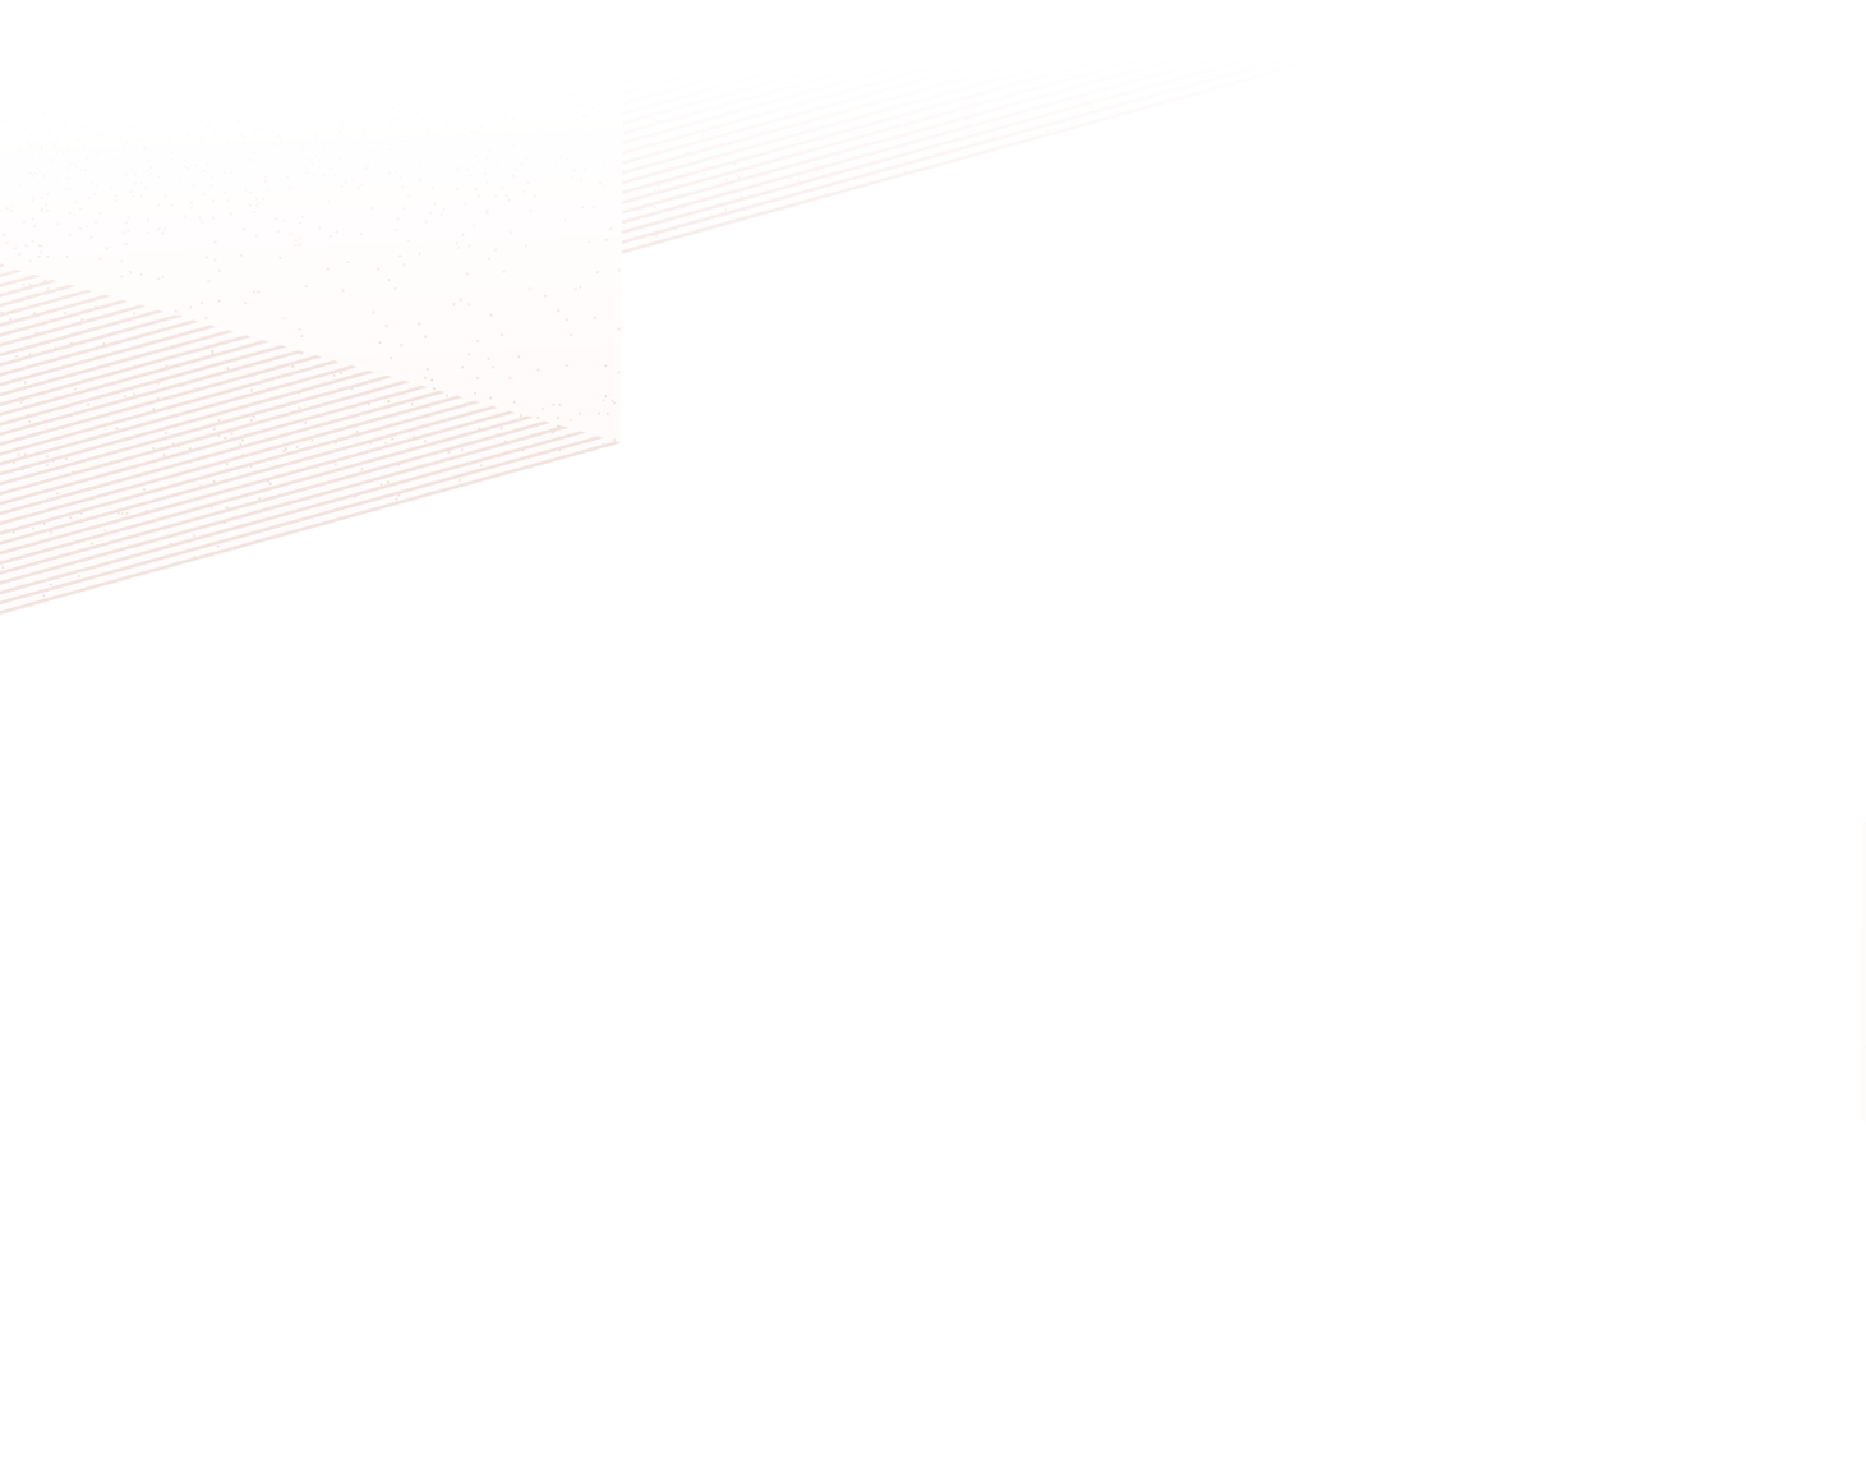
\includegraphics[width=\paperwidth,height=\paperheight]{./Couverture-these/MathSTIC/image-fond-MATHSTIC-dos.png}}}
\pagestyle{empty}
\vspace{-2cm}
%---------------------------%
\hspace{0.05cm}
\logouniversite{./Couverture-these/MathSTIC/logo-mathSTIC} %nom du fichier
%\scalelogouniversite{1.2} % mise a l'echelle de l'image (0.5=50% par exemple)
\hspace{1cm}\logoetablissement{./Couverture-these/MathSTIC/logo-etablissements/logoUR1}
\begin{tikzpicture}[remember picture,overlay,line width=0mm]
  \draw [draw=white,fill=white]
    (current page.north west) rectangle (\paperwidth,1);
  \node[xshift=0\paperwidth,yshift=2cm,text=white,font=\bf\Large] {
  
\includegraphics[scale=1.2]{./Couverture-these/MathSTIC/logo-mathSTIC}
  };
  \node[xshift=.45\paperwidth,yshift=2cm,text=white,font=\bf\Large] {
  
\includegraphics[scale=0.2]{./Couverture-these/MathSTIC/logo-etablissements/logoUR1}
  };
\end{tikzpicture}
\par\nobreak
\hspace{- 1.75cm}\noindent \textcolor{mathSTIC-Color}{\rule{\textwidth }{0.2cm}}  %\hspace{0.1cm}
\selectlanguage{french}
\section*{\textcolor{mathSTIC-Color}{Titre}: titre (en fran\c cais)..............}
\noindent \keywordsF{de 3 \`{a} 6 mots clefs}
\begin{multicols}{2}
\noindent \textbf{Resum\'{e} : }Eius populus ab incunabulis primis ad usque pueritiae tempus extremum, quod annis circumcluditur fere trecentis, circummurana pertulit bella, deinde aetatem ingressus adultam post multiplices bellorum aerumnas Alpes transcendit et fretum, in iuvenem erectus et virum ex omni plaga quam orbis ambit inmensus, reportavit laureas et triumphos, iamque vergens in senium et nomine solo aliquotiens vincens ad tranquilliora vitae discessit.
Hoc inmaturo interitu ipse quoque sui pertaesus excessit e vita aetatis nono anno atque vicensimo cum quadriennio imperasset. natus apud Tuscos in Massa Veternensi, patre Constantio Constantini fratre imperatoris, matreque Galla.
Thalassius vero ea tempestate praefectus praetorio praesens ipse quoque adrogantis ingenii. 
\end{multicols}




\hspace{- 1.75cm}\noindent \textcolor{mathSTIC-Color}{\rule{\linewidth}{0.2cm}}
\selectlanguage{english}
\section*{\textcolor{mathSTIC-Color}{Title}: title (en anglais)..............}
\noindent \keywordsE{de 3 \`{a} 6 mots clefs}
\begin{multicols}{2}
\noindent \textbf{Abstract: }Eius populus ab incunabulis primis ad usque pueritiae tempus extremum, quod annis circumcluditur fere trecentis, circummurana pertulit bella, deinde aetatem ingressus adultam post multiplices bellorum aerumnas Alpes transcendit et fretum, in iuvenem erectus et virum ex omni plaga quam orbis ambit inmensus, reportavit laureas et triumphos, iamque vergens in senium et nomine solo aliquotiens vincens ad tranquilliora vitae discessit.
Hoc inmaturo interitu ipse quoque sui pertaesus excessit e vita aetatis nono anno atque vicensimo cum quadriennio imperasset. natus apud Tuscos in Massa Veternensi, patre Constantio Constantini fratre imperatoris, matreque Galla.	Thalassius vero ea tempestate praefectus praetorio praesens ipse quoque adrogantis ingenii.
\end{multicols}
